% Based on template: http://www.maths.lth.se/matematiklth/exjobb/exjobbarresurs/index.html

\documentclass{IEEEtran}

\usepackage[smartEllipses]{markdown}  % For markdown
\def\markdownOptionOutputDir{build}  % Needed, see https://github.com/Witiko/markdown/issues/6#issuecomment-328699108

\usepackage[smartEllipses]{markdown}  % For markdown
\def\markdownOptionOutputDir{build}  % Needed, see https://github.com/Witiko/markdown/issues/6#issuecomment-328699108

\usepackage{array}
\usepackage{hyperref}
\usepackage{makecell}
\usepackage{comment}
\usepackage{xargs}
\usepackage{verbatim}
\usepackage{subfig}
\usepackage{booktabs}
\usepackage{changepage}
\usepackage{rotating, graphicx}
\usepackage{multirow}
\usepackage{pdflscape}
\usepackage{afterpage}
\usepackage[export]{adjustbox}
\usepackage[dvipsnames]{xcolor}
\usepackage[bottom]{footmisc}
\usepackage[colorinlistoftodos, prependcaption, textsize=tiny]{todonotes}

% References
\usepackage[backend=biber, style=numeric, sorting=none]{biblatex}
\usepackage{cleveref}

% Formatting
\setlength{\parindent}{0pt}
\setlength{\parskip}{1em}

% Encoding and languages
\usepackage[utf8]{inputenc}
\usepackage[english]{babel}
\usepackage[T1]{fontenc}        % För svenska bokstäver
%\usepackage[swedish]{babel}    %Svenska skrivregler och rubriker

% Graphics
\usepackage{epsfig}
%\usepackage[dvips]{graphics}

% For adding source captions to figures.
% From: https://tex.stackexchange.com/a/246285/36302
\newcommand{\source}[1]{\vspace{-0.3cm} \caption*{\footnotesize{Source: \textit{{#1}}}}}


\usepackage[english]{datetime2}
\DTMnewdatestyle{dashdate}{%
  \renewcommand{\DTMdisplaydate}[4]{\number##1-\DTMenglishshortmonthname{##2}-\number##3}%
  \renewcommand{\DTMDisplaydate}{\DTMdisplaydate}%
}
\DTMsetdatestyle{iso}

% From: https://tex.stackexchange.com/a/178806/36302
\newcommandx{\add}[2][1=]{\todo[linecolor=red, backgroundcolor=red!25, bordercolor=red, inline, #1]{\textbf{Add:} #2}}
\newcommandx{\unsure}[2][1=]{\todo[linecolor=red, backgroundcolor=red!25, bordercolor=red, #1]{\textbf{Unsure:} #2}}
\newcommandx{\change}[2][1=]{\todo[linecolor=blue, backgroundcolor=blue!25, bordercolor=blue, #1]{\textbf{Change:} #2}}
\newcommandx{\info}[2][1=]{\todo[linecolor=OliveGreen, backgroundcolor=OliveGreen!25, bordercolor=OliveGreen, #1]{\textbf{Info:} #2}}
\newcommandx{\improvement}[2][1=]{\todo[linecolor=Plum, backgroundcolor=Plum!25,bordercolor=Plum, #1]{\textbf{Improve:} #2}}
\newcommandx{\thiswillnotshow}[2][1=]{\todo[disable, #1]{#2}}

% Formatting
\setlength{\parindent}{0pt}
\setlength{\parskip}{1em}

\newcommand\myshade{85}
\colorlet{mylinkcolor}{violet}
\colorlet{mycitecolor}{YellowOrange}
\colorlet{myurlcolor}{Aquamarine}

\hypersetup{%
  linkcolor  = black, %mylinkcolor!\myshade!black,
  citecolor  = mycitecolor!\myshade!black,
  urlcolor = myurlcolor!\myshade!black,
  colorlinks = true,
}

% References
\bibliography{zotero}
\DeclareBibliographyCategory{cited}
\AtEveryCitekey{\addtocategory{cited}{\thefield{entrykey}}}

\defbibheading{notcited}{\section*{Further Reading}}

\title{%
    \small DRAFT \today \\
    \small The latest version is available at \href{https://erik.bjareholt.com/thesis/goaldocument.pdf}{erik.bjareholt.com/thesis/goaldocument.pdf}\\
    \large --- \\
    \large \par M.Sc. Thesis proposal\\
    \huge Classifying brain activity using low-cost biosensors and automated time tracking \\
}
\author{Erik Bjäreholt \\(erik@bjareho.lt, dat13ebj@student.lu.se)}
\date{\today}

\begin{document}
\maketitle

\begin{center}
\begin{tabular}{r l}
 Student & Erik Bjäreholt \\
 Supervisor & Markus Borg \\
 Examiner & Elizabeth Bjarnarson \\
 Start date & 1st October \\
 End date & 1st March \\
\end{tabular}
\end{center}

\setlength{\parskip}{0em}
\tableofcontents
\setlength{\parskip}{1em}

\listoftodos[Notes \& TODOs]

\begin{refsection}

\newcommand{\RQmain}{How well can data from low-cost EEG sensors be used to train a classifier separating software developers' device activities?}

\section{Summary}

This thesis project is about studying the viability of low-cost biosensors, EEG in particular, to determine the focus of software developers' attention. % or "differentiate between different activities that software developers engage in."

The primary research question we will answer is how well these sensors can be used to differentiate between different activities, similarly to how previous research has shown it to be possible to differentiate other tasks, such as prose vs code comprehension~\cite{fucci_replication_2019}.

This will be accomplished by measuring brain activity using EEG while simultaneously tracking what activity the developer is engaging in (such as writing code, reading documentation, or engaging with a non-work application such as social media). This will then be used to train a classifier to differentiate between the activities, in an attempt to determine if the EEG data contains sufficient information to approximate the focus of the developer's attention.

%\add{Note about how the active application is only an estimation of subject of the developers attention, despite it being used as labels for the dataset (a developer can be thinking about food while having the docs open, or be distracted by a notification that isn't captured)}

\section{Background}

People spend more time than ever using computing devices. Work, entertainment, and services, have been steadily moving online over the last few decades and this trend is expected to continue.
While several studies have been tracking how people spend time on their devices a wider study of how people's app usage is changing over time and how it varies with demographics, is not publicly available.

Furthermore, how different device activities affect the user behaviorally and neurologically is of interest for many areas of research, including:

\begin{itemize}
    \item psychological well-being, such as depression and social anxiety~\cite{selfhout_different_2009}\cite{shah_nonrecursive_2002}, stress~\cite{mark_stress_2014}, self-esteem, life satisfaction, loneliness, and depression~\cite{huang_time_2017}.
    \item the impact of screen time on children and adolescents~\cite{subrahmanyam_impact_2001}.
    \item attention span among media multitasking adults~\cite{mark_stress_2014}.
    \item enhancing personal productivity~\cite{kim_timeaware_2016}.
\end{itemize}

Understanding device use and the underlying cognitive processes are essential when designing for motivation, engagement and wellbeing in digital experiences~\cite{peters_designing_2018}.

This becomes especially relevant for knowledge workers, such as software developers, who spend the majority of their working time on computing devices.

%\add[inline]{Add connection to software developers}

\subsection{Automated time trackers}

Automated time-trackers have been developed for computing devices for various applications such as tracking productivity, managing excessive use of social networking sites (SNSs).

\subsubsection{Commercial use}

Companies like RescueTime~\cite{noauthor_rescuetime_nodate}, Hubstaff~\cite{noauthor_hubstaff_nodate}, and others offer automated time tracking as a service. These services let the user track their screen time by installing a program on their device which tracks the active application and sends the data to their servers for storage and analysis. The user can then view their data in a dashboard on the service's website. Some of these services, like RescueTime and Hubstaff, are marketed towards teams and professionals, who want to keep track of individual and team productivity.

However, these services have some issues for use by researchers and individuals alike. Notably, their collection of detailed and non-anonymized behavioral data into a centralized system bring significant privacy concerns, especially in cases where the data is shared with a team or an employer.

Other limitations of these services, such as low temporal resolution and limited event detail, cause additional issues for certain tasks that are timing-sensitive (such as ERPs), or preprocessing steps that can take advantage of high level of detail (like classifying activity).

\subsubsection{Research use}

Previous research has been published which used automated time trackers, such as TimeAware~\cite{kim_timeaware_2016} and ScreenLife~\cite{rooksby_personal_2016}. However, these previous contributions are --- like the commercial services --- not open source nor permissively licensed, and therefore not available for external research use nor further development.

\subsubsection{ActivityWatch}

The free and open source automated time tracker ActivityWatch~\cite{bjareholt_activitywatch_2020} addresses aforementioned issues with other software around source availability/licensing, privacy, temporal resolution, event detail, and cross-platform support.

\begin{figure}[h]
\centering
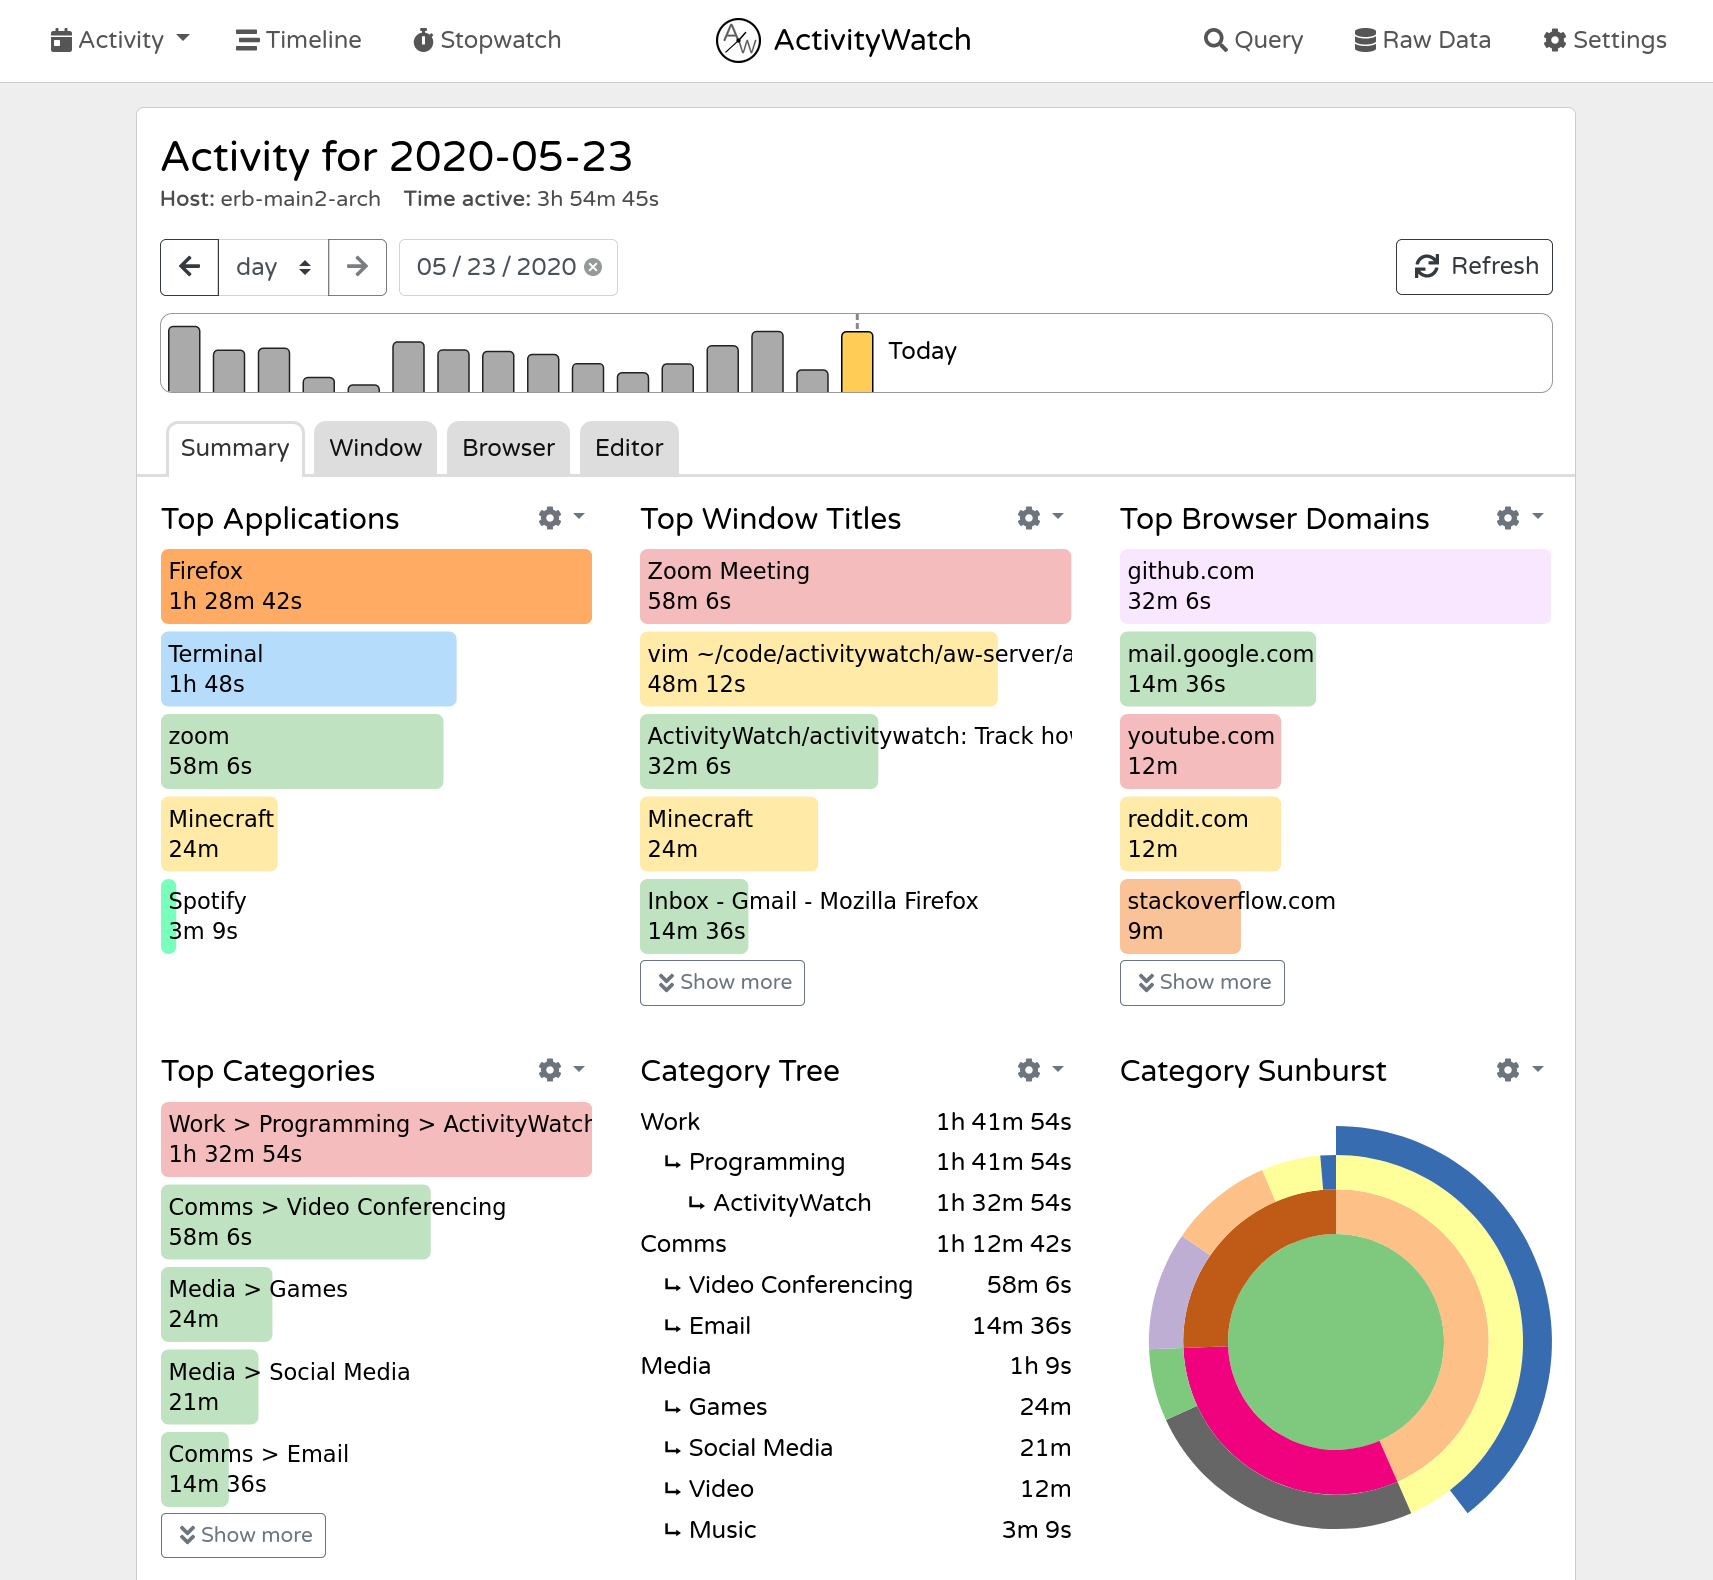
\includegraphics[width=8cm]{img/screenshot-aw-activity.png}
\caption{ActivityWatch activity dashboard. Showing top applications, window titles, browser domains, and categories.}\label{fig:aw}
\end{figure}

%With the advancement of Brain-Computer Interfaces, the relationship between device and brain activity is becoming even more tightly connected.

\subsection{Low-cost functional brain imaging}

Functional brain imaging methods such as fMRI, fNIRS, and EEG, have been used to study the relationship between cognitive or physical activity, and brain activity~\cite{floyd_decoding_2017}\cite{hong_classification_2015}\cite{fucci_replication_2019}. The more accurate methods such as fMRI are costly and inflexible/impractical for many uses.

However, the recent availability of low-cost biosensors such as EEG, HEG, and fNIRS, enables studying brain activity during real-life tasks. As an example it has been shown that it is possible to classify what task a participant is undertaking using fMRI~\cite{floyd_decoding_2017}, which has been replicated using EEG and low-cost biosensors~\cite{fucci_replication_2019}.

But they are not without their limitations --- among them a notably low signal-to-noise ratio~\cite{mcfarland_eeg-based_2017} --- yet visual evoked potentials (VEPs) have been shown to be sufficient for high-speed BCI applications~\cite{spuler_high-speed_2017}.

To combat the low signal-to-noise ratio, machine learning methods have been employed with varying degrees of success. Examples from previous research include Convolutional Neural Networks (CNNs), which have been successful in classifying time series in general~\cite{zhao_convolutional_2017}, and EEG data in particular~\cite{schirrmeister_deep_2017}. As well as Hierarchical Convolutional Neural Networks (HCNNs), which have been used for EEG-based emotion recognition~\cite{li_hierarchical_2018}.

% https://docs.openbci.com/citations

% List of functional brain imaging techniques:
%  - fMRI
%  - fNIRS
%  - EEG
%  - HEG

\section{Problem description, research goals and questions}

%\add[inline]{Needs an overarching value-adding goal/vision, relating to software engineering}

% Goal: Improve productivity of developers.

Knowledge workers in general, and software developers in particular, have varying degrees of productivity that is in part mediated by varying degrees of focus (or ``flow''). Physical devices which use device activity as an indicator of flow have been developed to reduce interruptions at work, and subsequently improve productivity~\cite{zuger_reducing_2017}.

%Methods such as biofeedback have been TODO \cite{neurosity}

Since EEG and other low-cost biosensors have been used to classify developers emotions~\cite{girardi_recognizing_2020} and comprehension tasks~\cite{fucci_replication_2019} we will investigate if they can also be used to classify which device activity the user is engaging in.

The goal of this project is therefore to investigate whether EEG and other low-cost biosensors can be used to improve the productivity of developers by studying the relationship between device activity and brain activity. This will be done in part by training a device activity classifier from EEG data. % This will be useful to future BCI applications where a command might be specific to a particular context.

We structure our goals according to the Goal-Question-Metric (GQM) paradigm. The goals are grouped into phases, which are explained in the Methodology section.

\begin{figure}[h]
\centering
\includegraphics[width=8cm]{img/gqm.png}
    \caption{Overview of the goals/phases (with a subset of the questions and metrics), structured according to the Goal-Question-Metric (GQM) paradigm.}\label{fig:gqm}
\end{figure}

\begin{markdown}
*Goal:* Characterize the EEG profile of different device activities, to inform the design of the multiple-subject experiment.

 - *Question:* Which device activities are the easiest to distinguish from each other based solely on EEG data?

    - *Metrics:* PSD, covariance matrix.

 - *Question:* Roughly how much data is required to characterize the EEG of a particular activity?

    - *Metrics:* Time for aggregated power spectra to converge.

 - *Question:* Which electrode placements (in the 10-20 system) are most suitable for the task?

    - *Metrics:* Covariance matrix.

 - *Question:* What is the baseline power spectra of device activity in general for a particular user?

    - *Metrics:* Power spectra.

 - *Question:* What are the power spectra of different activities (like work vs social media use)?

    - *Metrics:* Power spectra aggregated by device activity,

 - *Question:* Does the same activity consistently yield similar power spectral densities.

    - *Metrics:* Variance of the aggregated power spectra, both per user and across the entire group.

 - *Question:* Are any brain regions more strongly associated with certain activity? (similar to G2-Q3)

    - *Metrics:* Source estimation, covariance matrix.
\end{markdown}


\begin{markdown}
*Goal:* Develop a classifier for device activity from EEG data.

 - *Question:* Is the EEG data sufficient for building a accurate classifier for device activity?

    - *Metrics:* Classifier performance

 - *Question:* What classifier is suitable for the dataset?

    - *Metrics:* Accuracy, precision, F1 score of different classifiers.

 - *Question:* Which electrode placements/brain regions have the most predictive power?

    - *Metrics:* Source estimation, covariance matrix.
\end{markdown}

% Goal-Question-Metric
%
%   Goal:
%     Purpose: Measure
%     Issue: Difficulty of measuring
%     Object: Affective states
%     Viewpoint: during device use
%    - Develop a classifier (object) for device activity (process) and affective states (process)
%
%   Questions:
%    - Can device activity be classified from EEG data?
%    - Which device activities cause, or are caused by, which affective states?
%
%   Metrics:
%    - Classifier performance
%    - Statistical significance of relationship between device activity and affective states

%\subsection{Goals}

%\add{Goals}

%\begin{itemize}
%    \item{}
%\end{itemize}

\subsection{Research Questions}

%\add[inline]{Needs revision}

Can low-cost biosensors, like EEG, be used to\ldots

\begin{itemize}
    \item RQ1. \RQmain{}
    \item RQ2. Can we improve upon previous results in classifying code vs prose comprehension with EEG@? (more channels, improved classification pipeline)
   %\item Classify which device activity the user is engaging in?
   %\item Track emotional states during device use?
   %\item Measure focus/distractibility during various device activities?
   %\item Predict context switching?
   %\item Be used to measure flow?
   %\item What about measuring attention/distractibility?
\end{itemize}

\subsection{Challenges}

\begin{itemize}
    \item Low volume of EEG data collected (limited time for data collection)
    \item Limitations of low-cost EEG equipment (small number of channels)
    \item Orthogonal stimuli (eye movement/blinking, use of keyboard/mouse) which will contribute significant noise to the EEG readings not relevant for the classification task.
    %\item Scope creep (hopefully resolved by the time this document is finalized)
    %\item \add{More challenges}
\end{itemize}

\section{Methodology}

%\subsection{Data collection}

We will simultaneously collect EEG and device activity data from subjects during device use. EEG data will be collected with the 8-channel OpenBCI Cyton biosensing board and Ultracortex headset. Device activity data will be collected and categorized with ActivityWatch. The activity categories will be used to label the dataset so we can train the classifier.

Project planning and tasks will be managed using GitHub issues and the Kanban-like board provided by GitHub (GitHub Projects).

The project can be roughly split into three phases.

\begin{itemize}
 \item Run a single-subject pilot study and perform preliminary analysis.
 \item Design and run a multiple-subject study.
 \item Develop a classifier for device activity.
\end{itemize}

\subsection{Pilot study}

The purpose of the first phase is to collect a pilot dataset (using a single subject) to inform the design of the main study.

The main questions we want to answer in this phase are about the study design in phase 2. Such as to identify which activities are the easiest to distinguish using EEG and are thus best suited for further study. (See GQM for more questions to be answered)

\subsection{Multiple-subject study}

%\add[inline]{Suggestions of study designs from related work, such as Fucci et al}

The purpose of this phase is to collect data from controlled experiments with multiple subjects.

The experimental design and protocol will be partially drawn from previous research, including a study on recognizing developers emotions while programming~\cite{girardi_recognizing_2020}, along with a replication study utilizing EEG to classify code comprehension~\cite{fucci_replication_2019}.

\subsection{Develop classifier}

Using the data collected from the previous phase we will develop a classifier that classifies the category of device activity using EEG data.

Additionally, there are numerous available EEG datasets and challenges on Kaggle which will be used to inform the development of the classifier.



%Both approaches have their tradeoffs; for a single-subject study it'd be much easier to collect large amounts of data and have the data be consistent (electrode placement would be consistent). We also have access to a MRI scan of the single subject (me, the experimenter) which can be used to aid in EEG source localization. On the other hand, collecting data from several users ensures that any results we get or classifiers we build are generalizable.

%

%\subsection{Data analysis}

%% Use an emotion classifier to try to associate which activities are associated with which emotions.

%\add{}

\section{Scientific contributions}

\begin{itemize}
  \item Developing a classifier for device activity using low-cost biosensors.
  \item Identifying relationships between device activity and brain activity, as measured by EEG\@.
  \item Validating previous research on biofeedback in software engineering.
  \item Developing a framework for using ActivityWatch in research.
 %\item The addition of EEG-derived data to ActivityWatch. \unsure{Maybe out-of-scope, but obvious synergies so might not be extra work.}
 %\item The open source automated time-tracker ActivityWatch.
\end{itemize}


\section{Resources}

I have access to all the resources I need to perform the project, including:

\begin{itemize}
  \item OpenBCI Ultracortex headset and Cyton biosensing board (8 channels)
  \item Muse S EEG headset (4 channels)
  \item Access to significant CPU \& GPU compute capacity (helpful for machine learning)
 %\item HEGduino \unsure[inline]{Will it be of use?}
  \item 3--5 male test subjects who have given informed consent.
  \item ActivityWatch, an open source automated time tracker (already developed by the author, but never before used in a scientific publication)
  \item Resources from the NeuroTechX community, such as code notebooks.\cite{barachant_eeg-notebooks_2020}
  \item Open source software for EEG research such as MNE-Python~\cite{noauthor_mne-python_2020} and Brainflow~\cite{noauthor_brainflow_2020}.
  \item Publicly available EEG datasets on Kaggle.\cite{noauthor_search_nodate}
  \item Access to researchers who work with EEG at Lund University (at Department of Automatic Control and Department of Psychology)
  \item Computer
\end{itemize}

% References
%\bibbysegment{}
\printbibliography[category=cited]

% Further reading (uncited)
\nocite{*}
\defbibenvironment{bibnonum}
  {\list{}
     {\setlength{\leftmargin}{\bibhang}%
      \setlength{\itemindent}{-\leftmargin}%
      \setlength{\itemsep}{\bibitemsep}%
      \setlength{\parsep}{\bibparsep}}
  }
  {\endlist}
  {\item}
\printbibliography[notcategory=cited, env=bibnonum, heading=notcited]

\end{refsection}
\end{document}
